\chapter{Simulationsprogramm}\label{chap3}
Zur Bewältigung der in Kapitel \ref{sec:aufgabenstellung} beschriebenen
Aufgaben wurde das erweiterte Nagel-Schreckenberg-Modell \see{sec:erwmodel}
durch ein Matlabskript umgesetzt. Im Folgenden wird dieses Programm besprochen.

\section{Programmbedienung}
Die Abbildung \ref{programm} zeigt die graphische Oberfläche unseres Programmes. Im Folgenden wollen wir kurz alle Parameter erklären.
\begin{itemize}
\item[] \textbf{Länge der Straßenabschnitte:} Gibt die Anzahl der Zellen eines Straßenstückes an. Dabei würde die Zahl 100 die Straße in vertikaler als auch horizontaler Richtung in 201 Zellen aufteilen (zwei Straßenstücke plus Kreuzungspunkt).
\item[] Das Programm berechnet alle Simulationen mit vertikaler Dichte zwischen den Werten \textbf{Anfang} und \textbf{Ende} im Abstand der \textbf{Schrittweite}. Dabei ist mit vertikaler Dichte gemeint, wie viel Zellen in Prozent der vertikalen Straße mit Autos belegt sind. Analog die horizontale Dichte.
%\item[] \textbf{Start:}  Dieser Wert steht für die Anfangsdichte der vertikalen Straße in ... pro ... . 
%\item[] \textbf{Ende:} Gibt die Dichte am Ende von ... der vertikalen Straße in ... pro ... an.
%\item[] \textbf{Schrittweite:} Gibt 
%\item[] \textbf{Dichte horizontal:} Dieser Wert entspricht der horizontalen Dichte.
\item[] \textbf{Trödelwahrscheinlichkeit:} Gibt die Wahrscheinlichkeit $p \in [0,1]$ an mit der ein Autofahrer trödelt (siehe \hyperref[nagelschreckenberg_algo]{Nagel-Schreckenberg-Algorithmus}).
\item[] \textbf{Maximale Geschwindigkeit:} Entspricht der maximale Geschwindigkeit in Zellen pro Zeitschritt die ein Auto erreichen kann. 
\item[] \textbf{Zeitschritte:} Anzahl der Zeitschritte die berechnet werden sollen.
\end{itemize}

Im nachfolgenden wollen wir die Funktionalität der Buttons erläutern.
\begin{itemize}
\item[] \textbf{Generiere Zufallszahlen:} Dieser Button erzeugt eine zufällige Anfangsverteilung der Autos in Abhängigkeit der horizontalen und vertikalen Dichte. 
\item[] \textbf{Berechne:} Berechnet die Verkehrsflusssimulation in Abhängigkeit der Parameter. Dieser Button kann nur gedrückt werden, falls zuvor Zufallszahlen generiert wurden.
\item[] \textbf{Start Animation:} Dieser Button, der nur ausgeführt werden kann, wenn zuvor die Berechnung ausgeführt wurde, startet die Animation. 
\end{itemize}
Zum Schluss wollen wir noch die Bedeutung der Slider erklären.
\begin{itemize}
\item[] \textbf{Dichte der Animation:} Hier kann die vertikale Dichte ausgewählt werden, welche in der Animation gezeigt werden soll.
\item[] \textbf{Messpunkte:} Gibt die Zelle an, für die die Verkehrsflussdiagramme ausgewertet werden sollen. Dabei werden die Zellen horizontal von links nach rechts und vertikal von unten nach oben gezählt. D. h. der Wert 3 würde die Verkehrsflussdiagramme der dritten Zelle horizontal und der dritten Zelle vertikal liefern. 
\end{itemize}
Die einzelnen Diagramme werden in Kapitel 4 vorgestellt. 

\begin{figure}[H]%
\centering
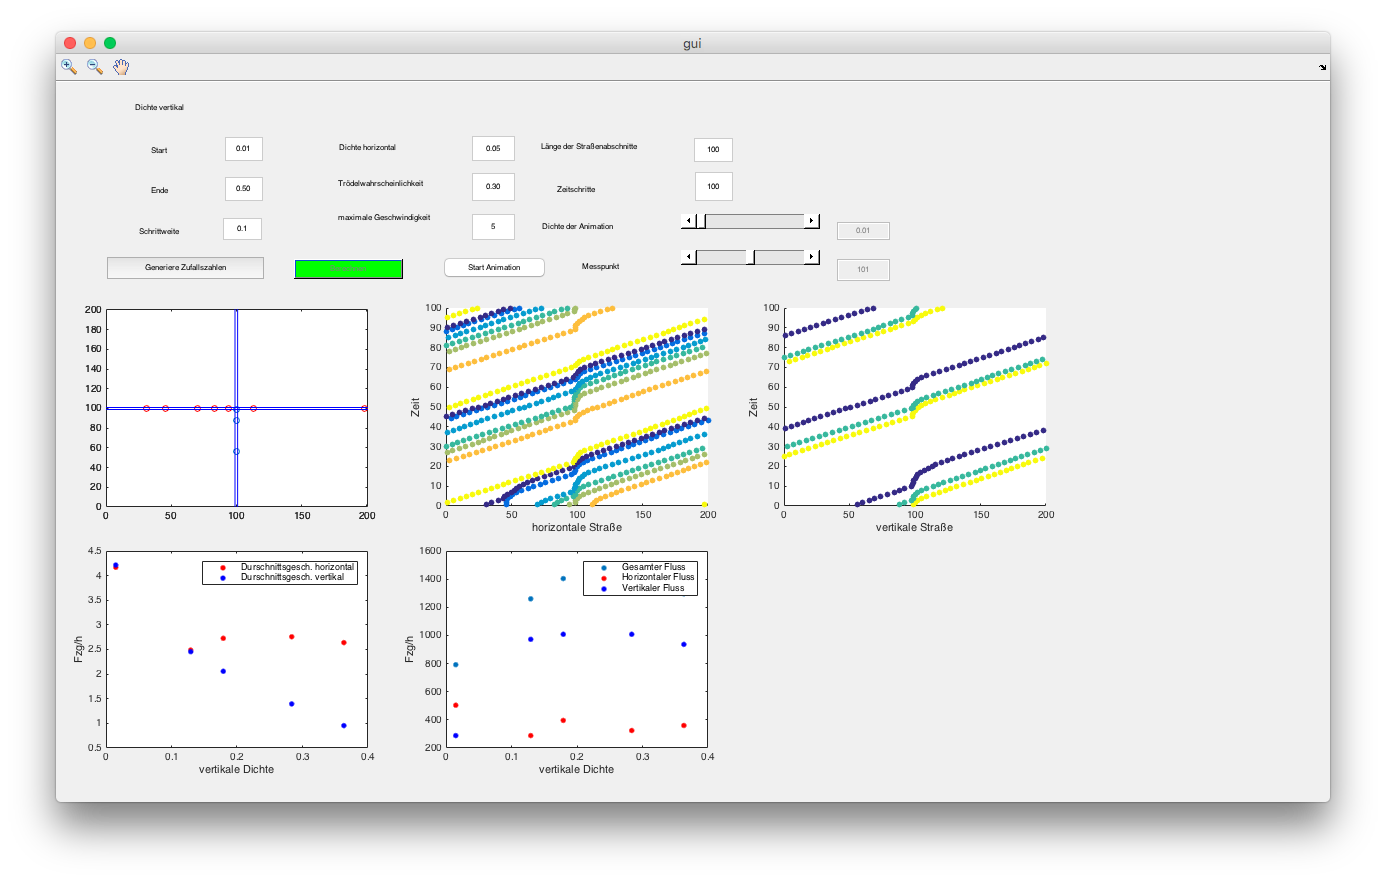
\includegraphics[width=17cm]{programm.png}%
\caption{Graphical User Interface}%
\label{pic:MaxFluss}%
\end{figure} \label{programm}
\noindent
\begin{flushright}
Autor: Julian Berndt
\end{flushright}

\section{Implementierung}
Von Beginn an wurde bei der Umsetzung darauf geachtet, wo immer es möglich war, auf Schleifen zu verzichten und stattdessen die in Matlab sehr effizient umgesetzten Matrixoperationen zu benutzen. Dies bedeutet vor allem, dass als grundlegende Datenstruktur Matrizen zu benutzen sind. 

\subsection{Die Daten: Kreuzung, Straße und Auto}
Eine Kreuzung besteht aus zwei Straßen, welche zur Vereinfachung als Horizontale und Vertikale bezeichnet werden. Beide Straßen haben den Kreuzungspunkt als gemeinsamen Straßenabschnitt. Dieser wird zweimal, in der Horizontalen und in der Vertikalen, abgespeichert. 
Weiter muss die Verkehrssituation für jeden Zeitpunkt abgespeichert werden und es sollen Autos langsam an den Kreuzungspunkt heranfahren. 
Für eine Straße werden demnach die folgenden Daten benötigt:
\begin{enumerate}
  \item Anzahl der Zellen \(N \in \mathbb{N}\)
  \item Anzahl der Zeitschritte, die Simuliert werden \(T \in \mathbb{N}\)
  \item Koordinate des Kreuzungspunktes \(c \in \{ 1, \ldots N \}\)
\end{enumerate}
Die Koordinaten entsprechen dabei den Zellennummern (von links nach rechts, bzw. unten nach oben fortlaufend durchnummeriert). 
Was noch fehlt, sind die Fahrzeuge selbst. Diese werden zu einem festen Zeitschritt beschrieben durch:
\begin{enumerate}
  \item Autonummer \(k \in \{ 1, \ldots, K \}, \; K \leq N\) 
  \item Geschwindigkeit \(v_k \in \{0, \ldots, v_{max} \}\)
  \item Position, d.h. Straße und Zellenkoordinate
\end{enumerate}
Dabei ist die Autonummer nur innerhalb einer Straße eindeutig. Dies ist ausreichend, da die Fahrzeuge nicht 
abbiegen, d.h. eine Straße nicht verlassen.
\\ \\
Insgesamt wird eine Straße durch zwei \(T \times N\)-Matrizen \(V, W\) beschrieben.
Die \(t\)-te Zeile dieser Matrizen stellt die Situation zur Zeit \(t\) (mit \(1 \leq t \leq T\)) dar, 
wobei die Spalten den Zellen entsprechen, in denen ein Auto stehen kann. 
Steht also zur Zeit \(t\) das Auto mit Nummer \(k\) (mit \(1 \leq k \leq K\)) und Geschwindigkeit \(v_k\) in der \(n\)-ten Zelle, 
so gilt \( W_{t, n} = k\) und \(V_{t, n} = v_k\). 
Ist andererseits zur Zeit \(t\) die \(n\)-te Zelle nicht belegt so gilt: \(W_{t, n} = 0 = V_{t, n}\).
Kurz gesagt speichert \(V\) die Geschwindigkeiten und \(W\) die Autonummern zu jeder Stelle und jedem Zeitpunkt.
\\ \\
Zu Beginn ist nur die jeweils erste Zeile, d.h. der erste Zeitschritt, initialisiert und die anderen Matrixeinträge
sind mit Null vorbelegt. Dabei werden die Autos mit zufälliger Position und Geschwindigkeit gemäß
einer eingestellten Dichte \(\rho\) gesetzt. Dies erledigt die Funktion \begin{code}init\_street.m \end{code} \footnote{Die tatsächliche 
Implementierung ist etwas allgemeiner. So können beispielsweise mehrere Kreuzungen und auch andere
Hindernisse eingebaut werden, an denen Autos nur mit Geschwindigkeit \(1\) vorbeifahren können. Der Rest des Programms 
beschränkt sich jedoch auf den Spezialfall einer Kreuzung.}:
\begin{enumerate}
  \item Übergabeparameter
    \begin{enumerate}
      \item Anzahl der Zellen bis zur Kreuzung \(n\) 
      \item Verkehrsdichte \(\rho\)
      \item Simulationsdauer \(T\)
      \item Höchstgeschwindigkeit \(v_{max}\) 
    \end{enumerate}
  \item Rückgabewerte
    \begin{enumerate}
      \item Koordinate der Kreuzung \(c\) 
      \item Geschwindigkeitsmatrix \(V\) von Dimension \(T \times N\) \\ mit \(N := 2n+1\)
      \item Autonummernmatrix \(W\) von Dimension \(T \times N\) 
    \end{enumerate}
\end{enumerate}
Die erzeugte Straße ist also \(2n+1\) Zellen lang und der Kreuzungspunkt befindet sich  in der Mitte, d.h. an der 
Koordinate \(c = n+1\). Im weiteren Programmverlauf wird jedoch nur der Rückgabewert \(c\) ausgewertet, so dass die Kreuzung
leicht verschoben werden kann. Hier ein Beispiel für \(n=2\) und \(T=2\):
\[
  V = 
  \begin{bmatrix}
    v_1& 0& 0& v_2& v_3 \\
    0& 0& 0& 0& 0
  \end{bmatrix}, \;
  W = 
  \begin{bmatrix}
    1& 0& 0& 2& 3 \\
    0& 0& 0& 0& 0
  \end{bmatrix}, \;
  c = 3
\]
Es stellt sich die Frage, ob man auch mit einer Matrix auskommt. Eine Möglichkeit besteht darin sich nur die Geschwindigkeitsmatrix 
zu speichern und freie Straßenabschnitte mit \(-1\) zu kodieren. Dann ist es jedoch nicht ohne Weiteres möglich den Zustand eines bestimmten Autos über
mehrere Zeitschritte hinweg zu verfolgen, vor allem wenn zukünftige Erweiterungen beispielsweise Überholmanöver der Autos erlauben sollen.

\subsection{Der Algorithmus: Beschleunigen, Bremsen und Trödeln}
Wir betrachten zunächst die Vertikale und die Horizontale getrennt, d.h. das Folgende wird
auf beide Straßen angewendet.
\\ \\
Um den nächsten Zeitschritt berechnen zu können, muss man für jedes Auto wissen, wie viele freie Zellen 
in Fahrtrichtung vorhanden sind. Dabei reicht es \(v_{max}\) Zellen vorauszuschauen. 
Eine Zelle ist genau dann nicht frei, wenn sie ein Auto beinhaltet oder
die Kreuzungszelle ist. Hierfür wurde die Funktion \code{freeCells.m} geschrieben:
\begin{enumerate}
  \item Übergabeparameter
    \begin{enumerate}
      \item Straßenbelegung \(w_t\) zum Zeitpunkt \(t\),  also die Zeile \(t\) der Matrix \(W\)       
      \item Koordinate der Kreuzung \(c\) 
      \item Maximale Geschwindigkeit \(v_{max}\)
    \end{enumerate}
  \item Rückgabewerte
    \begin{enumerate}
      \item Vektor \(u\) der Länge \(N\) mit \(u_i \in \{0, \ldots, v_{max} \}\) ist Anzahl der freien 
        Zellen in Fahrtrichtung ab Zelle \(i\), also \(j := i + u_i + 1 \Rightarrow W_{t,j} \neq 0 \lor j = c\).
    \end{enumerate}
\end{enumerate}
Nun kann entsprechend gebremst oder beschleunigt werden. So wird für alle mit Autos belegten Zellen \(i\)
die neue Geschwindigkeit auf \(u_i\) gesetzt falls \(u_i < v\) und auf \(v\) falls \(u_i \geq v\) mit
\( v := \min\{ v_{max}, V_{t,i}+1 \}\).  
Dafür wurde die Funktion \code{adjustSpeed.m} geschaffen, die intern \code{freeCells.m} benutzt:
\begin{enumerate}
  \item Übergabeparameter
    \begin{enumerate}
      \item Straßenbelegung \(w_t\) zum Zeitpunkt \(t\),  also die Zeile \(t\) der Matrix \(W\)       
      \item Geschwindigkeiten \(v_t\) zum Zeitpunkt \(t\),  also die Zeile \(t\) der Matrix \(V\)       
      \item Koordinate der Kreuzung \(c\) 
      \item Maximale Geschindigkeit \(v_{max}\)
    \end{enumerate}
  \item Rückgabewerte
    \begin{enumerate}
      \item Vektor \(\hat{v}\) der Länge \(N\) mit \(\hat{v}_i\) ist neue Geschwindigkeit des Autos der Zelle \(i\)
    \end{enumerate}
\end{enumerate}
Insbesondere bleiben Autos zunächst vor der Kreuzung stehen. Nach dem Aufruf von \code{adjustSpeed.m} für die
Horizontale und die Vertikale kann also entschieden werden, ob ein Auto den Kreuzungspunkt betreten darf. 
Dazu wird überprüft, ob die Kreuzung frei. Es bezeichne \(W^h\), \(\hat{v}^h\) und \(c^h\) 
die Autonummernmatrix, den angepassten Geschwindigkeitsvektor und den Kreuzungspunkt der Horizontalen, sowie
\(W^v\), \(\hat{v}^v\), \(c^v\) das selbige für die Vertikale. Ist die Kreuzung frei, so muss demnach gelten: 
\[W^h_{t,c^h} = 0 = W^v_{t,c^v}\] 
Ist dies der Fall und steht auf der Vertikalen
ein Auto vor der Kreuzung 
\[W^v_{t,c^v-1} \neq 0\] so darf dieses Auto über die Kreuzung mit Geschwindigkeit \(1\). 
Es wird also 
\[\hat{v}^v_{c^v-1} = 1\] 
gesetzt. Steht auf der Vertikalen kein Auto vor der Kreuzung, 
aber auf der Horizontalen 
\[W^h_{t,c^h-1} \neq 0\]
so wird dessen angepasste Geschwindigkeit auf \(1\) gesetzt. 
Damit ist die Regel \textit{Rechts vor Links} umgesetzt.
Da dies in einem Zeitschritt abläuft fahren die Autos mit Geschwindigkeit \(1\) über die Kreuzung.
\\ \\
Hiernach wird für beide Straßen einzeln getrödelt (\code{linger.m}), also mit einer festgesetzten Wahrscheinlichkeit werden
die Geschwindigkeiten in \(\hat{v}\) um eine Einheit reduziert. 
Schließlich erfolgt durch die Funktion \code{shift.m} für beide Straßen einzeln die Berechnung des nächsten Zeitschrittes, 
also der Zeile \(t+1\) in den Matrizen \(V,W\) gemäß der Geschwindigkeiten \(\hat{v}\).
\\ \\
Der hier beschriebene Vorgang zur Berechnung der Zeitschritte ist in der Funktion \code{nagelschreckenberg.m} umgesetzt, 
sodass über die oben beschriebene GUI mit verschiedenen Startbedingungen (z.B. Trödelwahrscheinlichkeiten, Verkehrsdichten, Streckenlängen) experimentiert werden kann.

\begin{flushright}
Autor: Philipp Schwarz
\end{flushright}
